

\section{The Large Hadron Collider}

The Large Hadron Collider (LHC) is the world's largest and most powerful particle collider\cite{ipac11:lamont}. It was built by the European Organization for Nuclear Research (CERN) between 1998 and 2008 in collaboration with scientists and engineers from over 100 countries, as well as hundreds of universities and laboratories. It lies in a tunnel 27 km in circumference and as deep as 175 m beneath the France-Switzerland border near Geneva, Switzerland, which was originally digged for the Large Electron Positron Collider (LEP). 

\begin{figure}[tbh!]
	\centering
	\begin{tabular}{cc}
		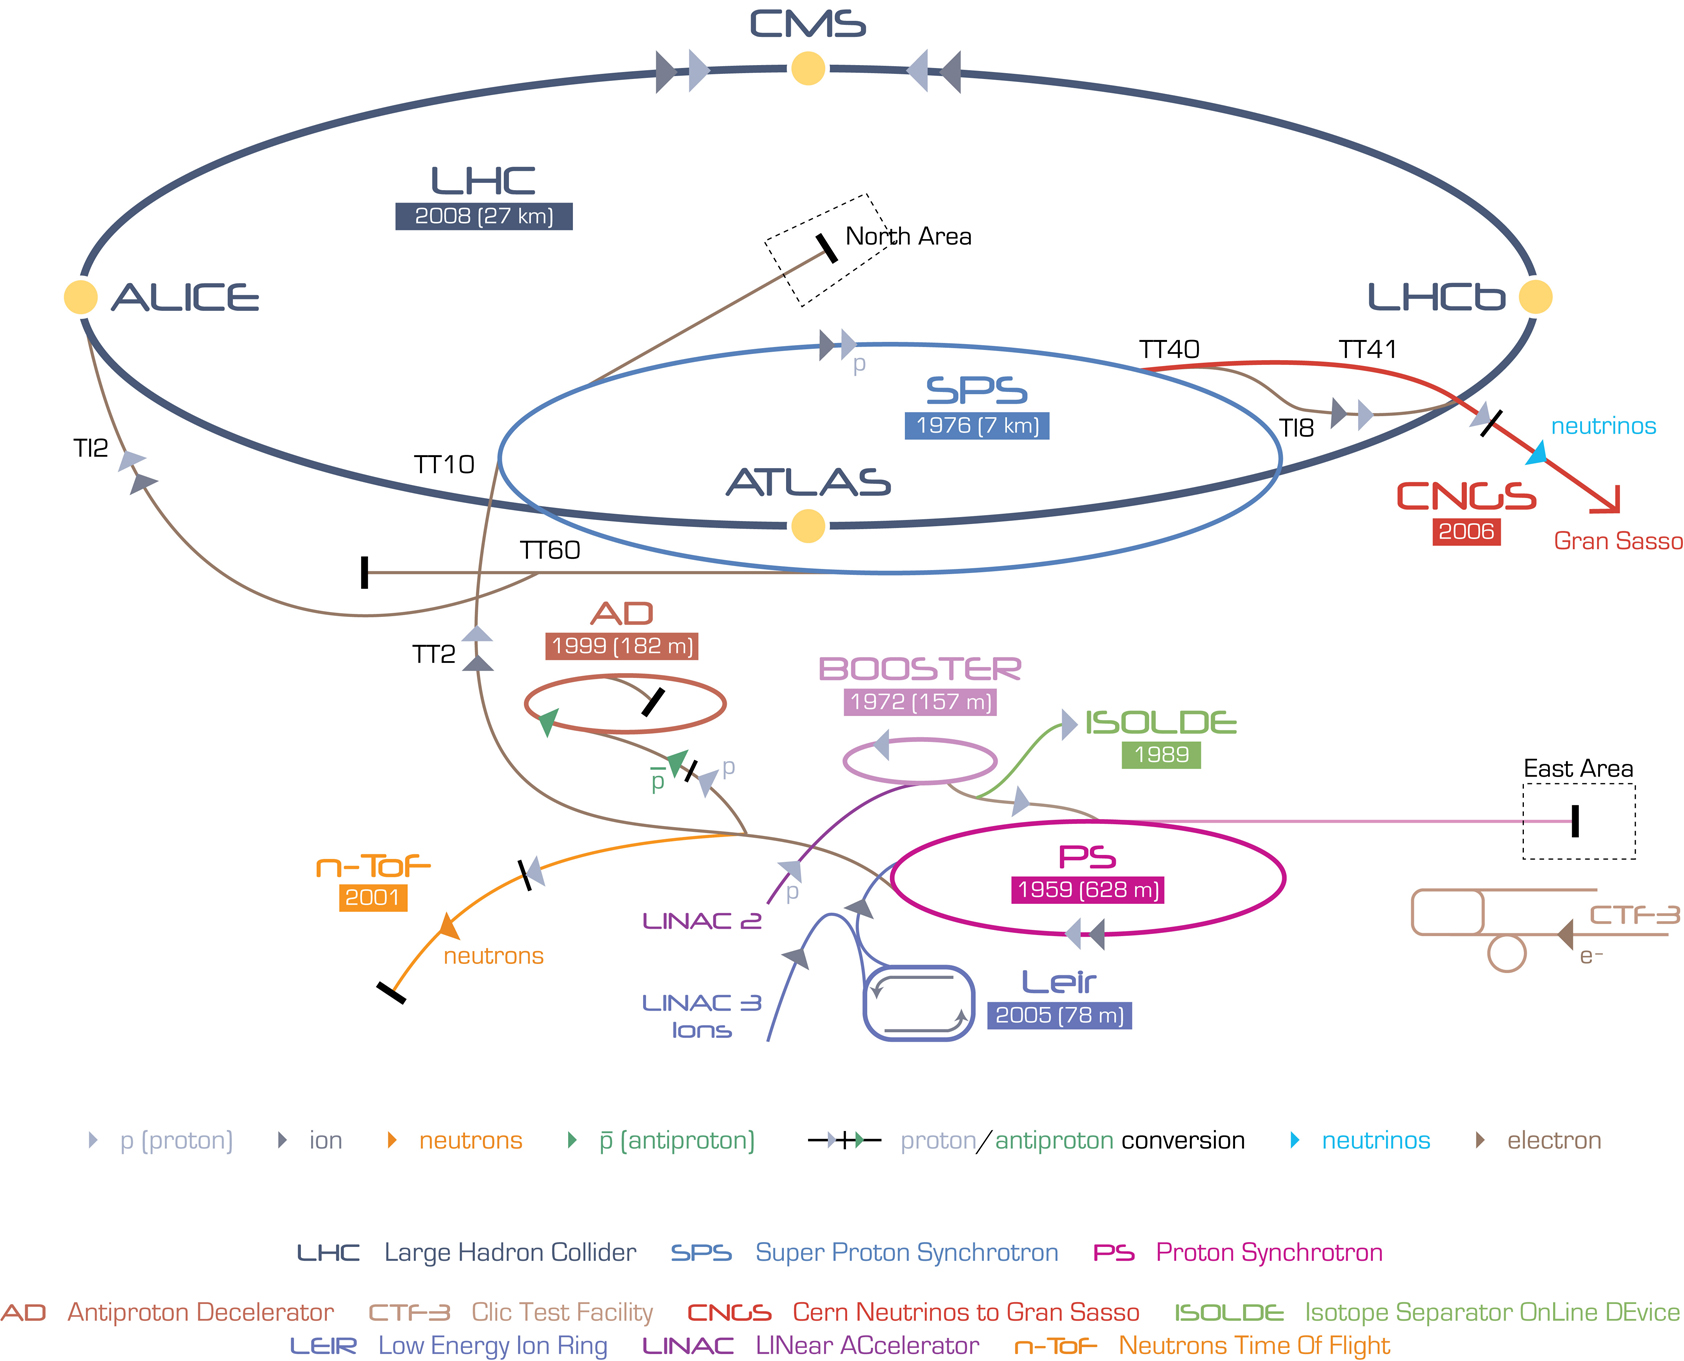
\includegraphics[width=0.75\textwidth]{detector/pics/CERN_complex.jpg}
	\end{tabular}
	\caption{Schematic view of the LHC with its four big experiments. Also shown are the pre-accelerators, as well as several other experiments operated at CERN \cite{Collider:1998498}.}
	\label{fig:CERN_complex}
\end{figure}

It is a proton-proton collider and consists of two rings with counter-rotating beams, that intersect each other at four interaction points. The proton beams are ramped up to the energy of 450 GeV by a chain of pre-accelerators, and are then injected into the LHC ring ( \autoref{fig:CERN_complex}). LHC first data taking period, also called \textit{Run1}, started on March 2010 with an initial energy per beam of 3.5\tev (7\tev in total), rising to 4\tev per beam (8\tev in total) in 2012. The shutdown in 2013 was followed by two years of technical upgrades after which the LHC restarted "\textit{Run2}" with a total center of mass energy of 13\tev. The design luminosity L is $10^{34}$ \ensuremath{\text{cm}^{-2}\text{s}^{-1}} and has been reached in June 2016, with a bunch crossing taking place every $25 \text{ns}$. \autoref{fig:LHC_xsec} shows the total cross section prospects for LHC in comparison with several Standard Model processes. In 2012 LHC delivered a total luminosity of 23.30\invfb as shown on \autoref{fig:lumi_2012}. The delivered luminosity accounts for the luminosity delivered from the start of stable beams until the LHC requests CMS to turn off the sensitive detectors to allow a beam dump or beam studies. Given is the luminosity as determined from counting rates measured by the luminosity detectors. These detectors have been calibrated with the use of the van-der-Meer beam-separation method, where the two beams are scanned against each other in the horizontal and vertical planes to measure their overlap function \cite{CMS:LumiPublicResults}.

\begin{figure}[tbh!]
	\centering
	\begin{tabular}{cc}
		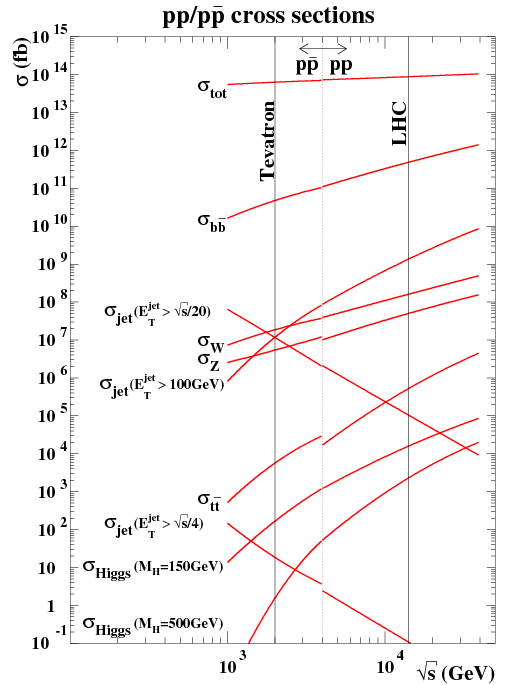
\includegraphics[width=0.75\textwidth]{detector/pics/LHC_xsec.png}
	\end{tabular}
	\caption{Production cross-sections for several representative processes at hadron colliders as a function of the machine's center-of-mass energy \cite{Weiglein:2004hn}}
	\label{fig:LHC_xsec}
\end{figure}


Several experiments are hosted at the LHC. ATLAS (A Toroidal LHC ApparatuS) \cite{det::ATLAS} and CMS (Compact Muon Solenoid) \cite{Chatrchyan:2008zzk} are multi-purpose detectors, aiming at Standard Model physics, Higgs searches, and physics beyond the Standard Model. LHCb \cite{det::LHCb} is dedicated to b-quark physics and the related problem of CP violation the matter-antimatter asymmetry in the universe. As the LHC can also be run in heavy ion (lead-lead) collision mode. One experiment, ALICE (A Large Ion Collider Experiment) \cite{det::ALICE}, focuses on strongly interacting matter and quark-gluon plasma. Finally, another two experiments, LHCf \cite{Adriani:2008zz} and TOTEM (TOTal Elastic and diffractive cross section Measurement) \cite{Anelli:2008zza} are designed to study the total proton-proton interaction cross-section. The sites for each of the previously mentioned experiments are shown in \autoref{fig:CERN_complex}. 

\begin{figure}[tbh!]
	\centering
	\begin{tabular}{cc}
		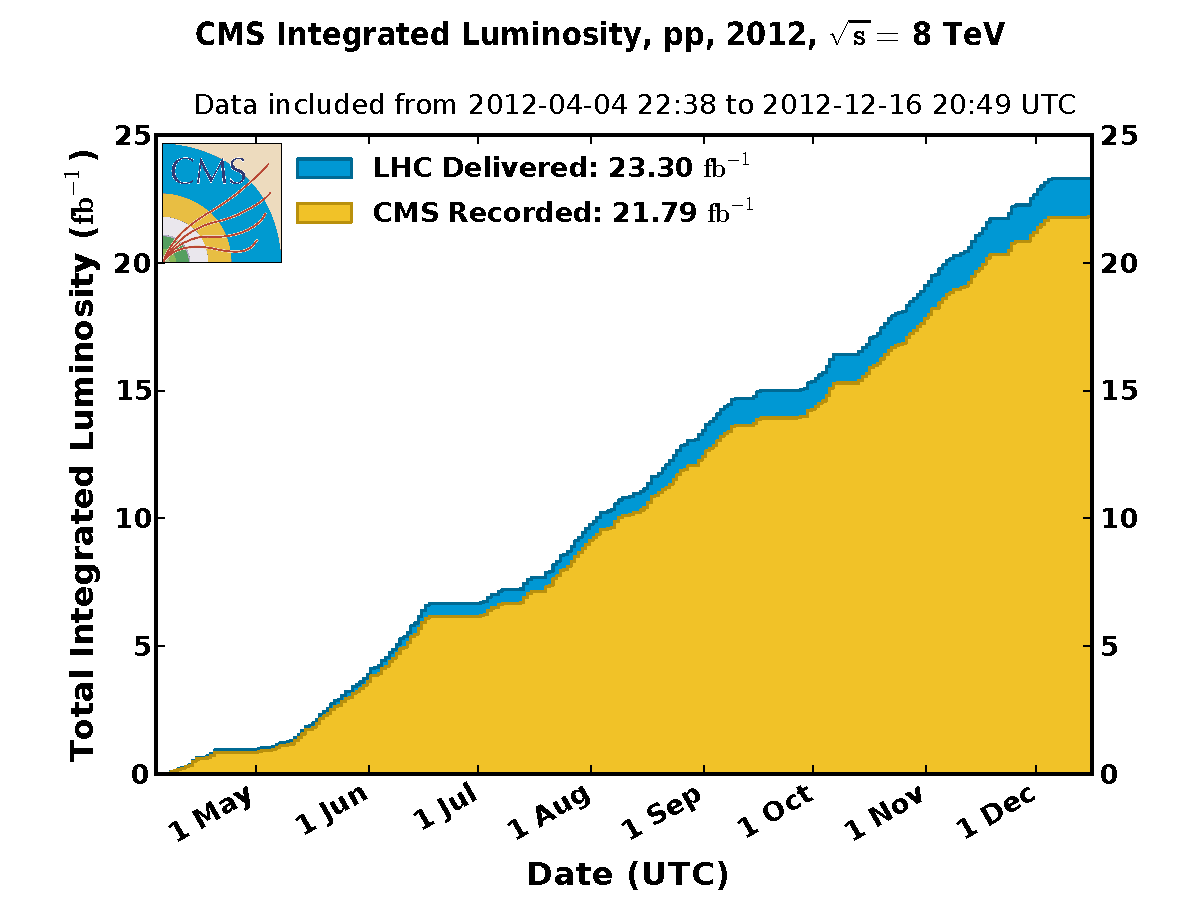
\includegraphics[width=0.75\textwidth]{detector/pics/int_lumi_per_day_cumulative_pp_2012.pdf}
	\end{tabular}
	\caption{Cumulative luminosity as function of time delivered to (blue), and recorded by CMS (orange) during stable beams and for p-p collisions at 8 TeV centre-of-mass energy in 2012 \cite{CMS:LumiPublicResults}.}
	\label{fig:lumi_2012}
\end{figure}

\clearpage

\section{The CMS experiment}

The Compact Muon Solenoid is a "general purpose" experiment placed at Point 5 along the LHC ring. The experiment has a cylindrical geometry and is divided in two main sections: the lateral section, called Barrel and the remaining ones called Endcaps (\autoref{fig:CMS_apparatus}).   
CMS was designed to fulfill among others the following important research tasks:
\begin{enumerate}
	\item Search for the Higgs Boson
	\item Search for physics beyond the standard model
\end{enumerate}
Those tasks combined with the LHC design specifications require a detector with the following characteristics:
\begin{itemize}
	\item High granularity and response;
	\item High radiation damage resistance;
	\item Good performances in the reconstruction of the $\mu$ particle charge, momentum and invariant mass;
	\item Good $\tau$ particle reconstruction efficiency;
	\item Good jet and b-jet reconstruction efficiency;
	\item High resolution on the combined reconstruction of electrons and photons;
	\item Great phase-space coverage of pseudo-rapidity $|\eta| < 5$;
	\item Good resolution in the missing transverse energy reconstruction.
\end{itemize} 

The CMS detector has a length of $24$ m and a diameter of $14.6$ m for a total weight of $14500 \text{t}$. The experiment is made of several sub-detectors placed concentrically around the interaction point, each one providing complementary measurements (\autoref{fig:CMS_slice}). Particles coming from the interaction point first go through the tracking system which measures the position of charged particles traveling through its layers. The calorimeters are placed right outside the tracking system and are capable of measuring the particles energy deposits. The Electromagnetic Calorimeter (ECAL) measures the energy of electrons and photons, the Hadronic Calorimeter (HCAL) measures the energy of “hadrons”, particles made of quarks and gluons.
 
Measurements with high resolution standards require high magnetic fields, therefore the CMS collaboration made the important choice to adopt superconducting technology for the experiment magnet. All previously introduced sub-detectors are contained inside the solenoid magnet. All particles except for muons and neutrinos are absorbed by the calorimeters. Outside the magnet there are the muon chambers witch identify muon particles and measure their momentum.

\begin{figure}[tbh!]
	\centering
	\begin{tabular}{cc}
		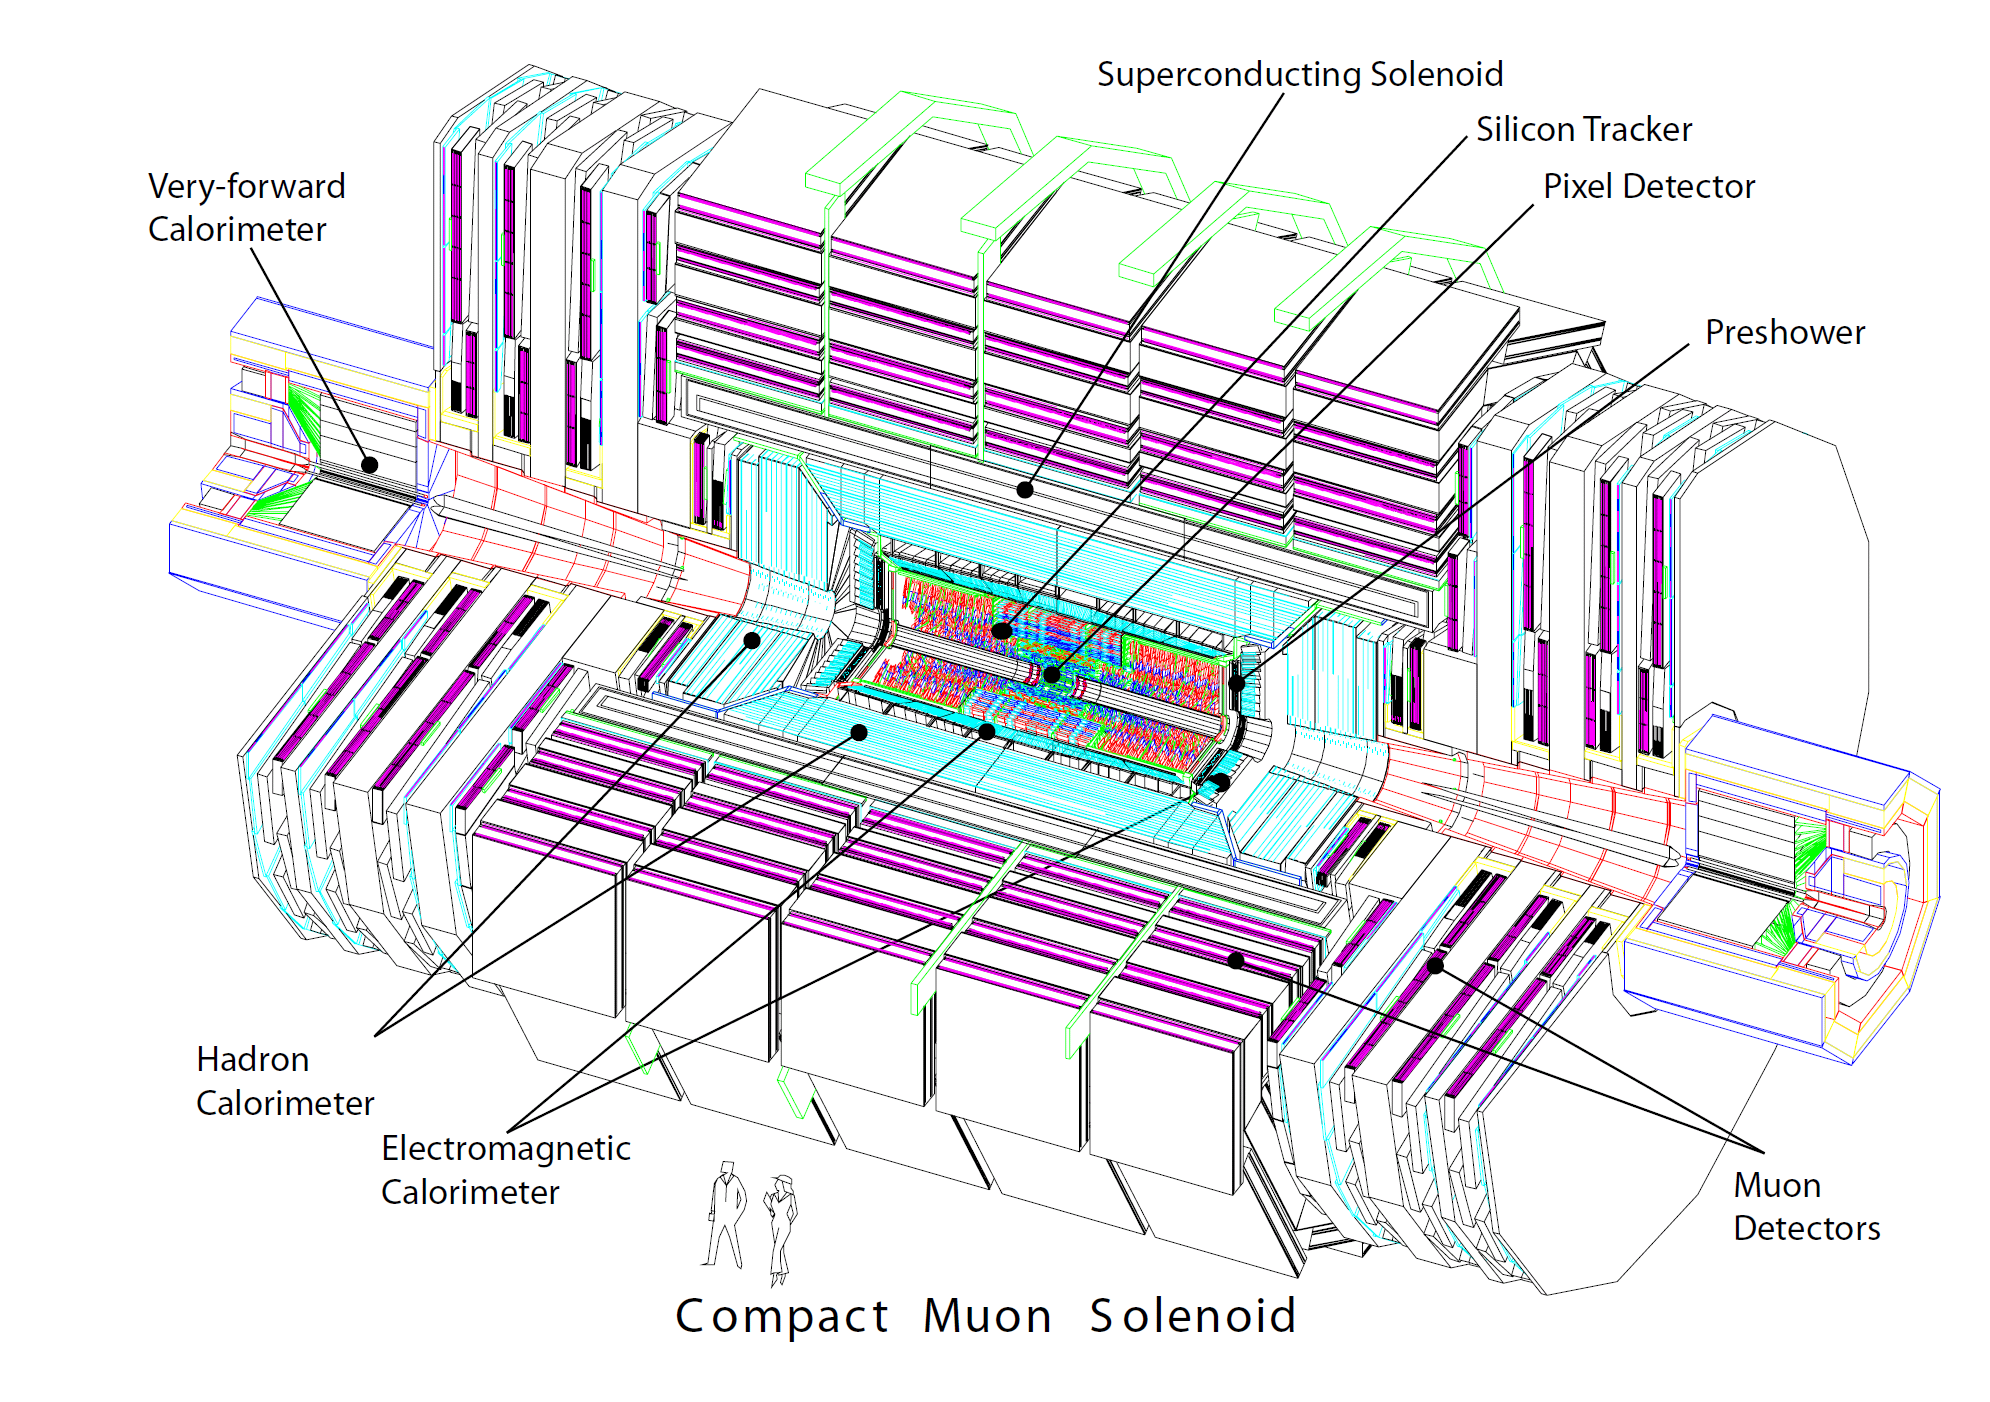
\includegraphics[width=0.75\textwidth]{detector/pics/CMS_apparatus.png}
	\end{tabular}
	\caption{An exploited view of the CMS detector.}
	\label{fig:CMS_apparatus}
\end{figure}

\begin{figure}[tbh!]
	\centering
	\begin{tabular}{cc}
		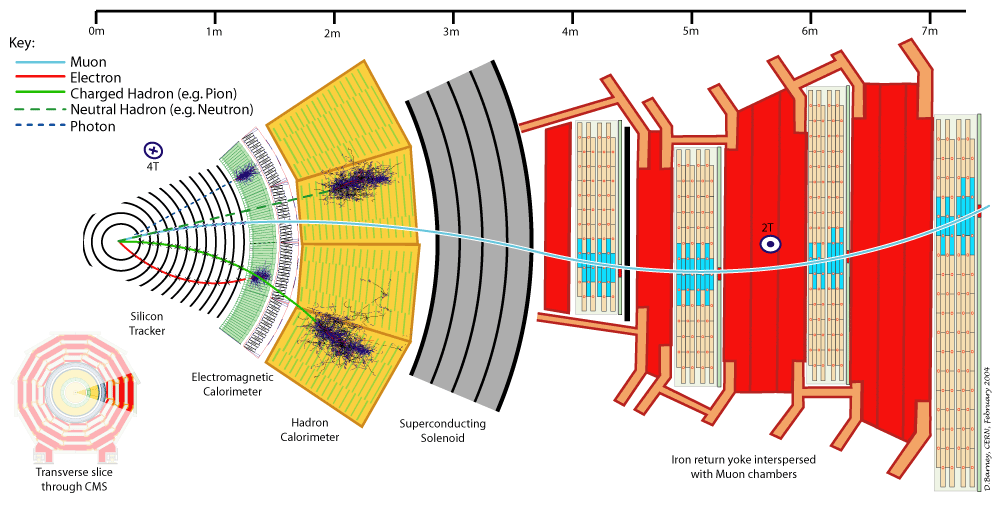
\includegraphics[width=0.75\textwidth]{detector/pics/CMS_slice.png}
	\end{tabular}
	\caption{Longitudinal section of the CMS detector showing the different detectors components and position.}
	\label{fig:CMS_slice}
\end{figure}

\clearpage

\subsection{The magnet}

The precision requirements of the muon chambers in order to distinguish unambiguously at $1$ TeV/c the muon charge is $\Delta p / p \approx 10\%$ and therefore requires of a magnetic field with high bending power. The main features of the CMS solenoid are the use of a high-purity aluminium-stabilised conductor and indirect cooling (by a thermosyphon), together with full epoxy impregnation.

The CMS magnet is a large superconducting solenoid with an inner bore of 5.9 m and a length of 12.9 m.  This good length-to-radius ratio is necessary to ensure good momentum resolution in the forward region as well. Its size is enough to contain the tracking system, the electromagnetic calorimeter and the hadronic calorimeter. 

The high magnetic field of $3.8$ T is generated by a current of 19.5 kA going through 2168 coil turns. An important parameter for this superconducting magnets design is the value of the hoop stress of 64 atm produced by the magnetic pressure due to the Lorentz force. The amount of total energy stored by the superconducting magnet is of 2.7 GJ.

%\begin{figure}[tbh!]
	%\begin{center}
		
	%\begin{tabular}{ | l | l |}
			%\hline
			%Field & 4 T \\ \hline
			%Inner Bore & 5.9 m \\ \hline
			%Length & 12.9 m \\ \hline
			%Number of Turns & 2168  \\ \hline
			%Current & 19.5kA   \\ \hline
			%Stored Energy & 2.7 GJ  \\ \hline
			%Hoop Stress & 64 atm \\
			%\hline
		%\end{tabular}
		%\caption{Parameters of the CMS superconducting solenoid.}
		%\label{table:CMS_magnet}
	%\end{center}
%\end{figure}

\subsection{Inner tracking system}

The Inner Tracking systems reconstructs the track of charged particles and measures their momentum. In order to meet the design requirements of a compact design and high reconstruction efficiency ($95\%$ for high momentum $\mu$ particles) the main detector material is silicon.
The detector can be divided in three parts:
\begin{itemize}
	\item Close to the interaction point are the pixel detectors since the particle flux is very high. Each pixel is $100\times150\mum^{2}$ wide;
	\item In the intermediate region ($20 < r < 55\cm$) the particle flux is low enough to allow the usage of silicon micro-strips, each cell has the minimum size $10\cm \times 80\mum$;
	\item In the outermost region ($r > 55\cm$), the particle flux is low enough to allow bigger size micro-strips with size of $25\cm \times 180 \mum$ 
\end{itemize}

A section of the whole inner tracking apparatus on the z-plane can be seen in \autoref{fig:Pixel_zview}. Close to the interaction point three pixel-layers are placed at radial distances of $4.7$, $7.3$ and $10.2\cm$. In the Barrel region the silicon micro-strips are placed at a radial distance between $20$ and $110\cm$. The forward region has instead two pixel and nine micro-strips layers. The barrel micro-strip section is divided in two different parts: the innermost and the outermost one. There are an additional three Inner Disks in the transition region between the Barrel and Endcap parts, on each side of the Inner Barrel. The total area of the pixel detector is $\approx 1\m^{2}$, whilst that of the silicon strip detectors is $200\m^{2}$, providing coverage up to $|\eta| < 2.4$. The inner tracker comprises 66 million pixels and $9.6$ million silicon strips. The silicon pixels grants a precision of $10\mum$ on the $(x,y)$ transverse plane and of $20\mum$ on the z axis. The resolution of the silicon micro-strips depends on each cell thickness, with a minimum value of $ 55\mum$ for the traverse plane. The overall layout apparatus is illustrated in \autoref{fig:Tracker_layout}.


\begin{figure}[tbh!]
	\centering
	\begin{tabular}{cc}
		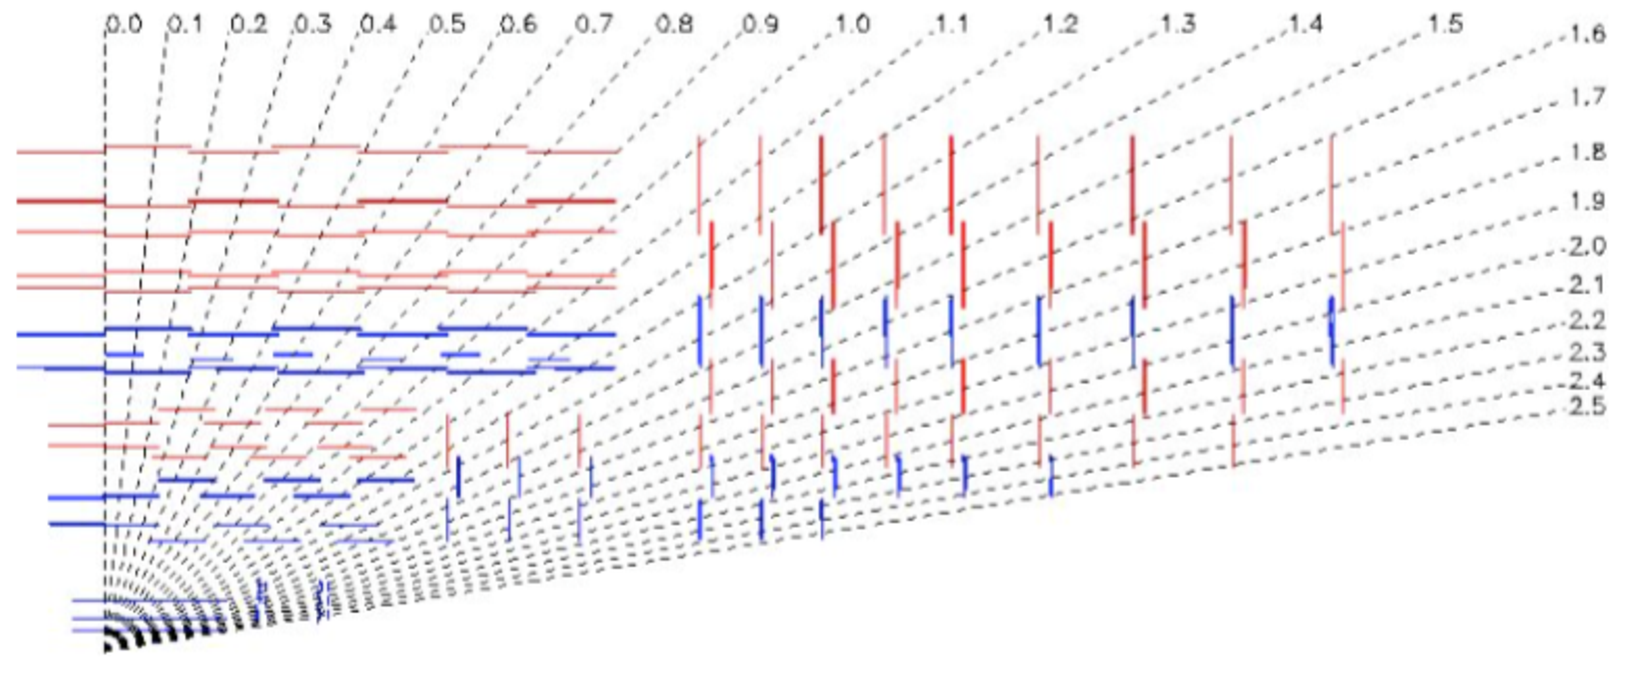
\includegraphics[width=0.75\textwidth]{detector/pics/Pixel_zview.pdf}
	\end{tabular}
	\caption{The tracker layout (1/4 of the z view).}
	\label{fig:Pixel_zview}
\end{figure}

\begin{figure}[tbh!]
	\centering
	\begin{tabular}{cc}
		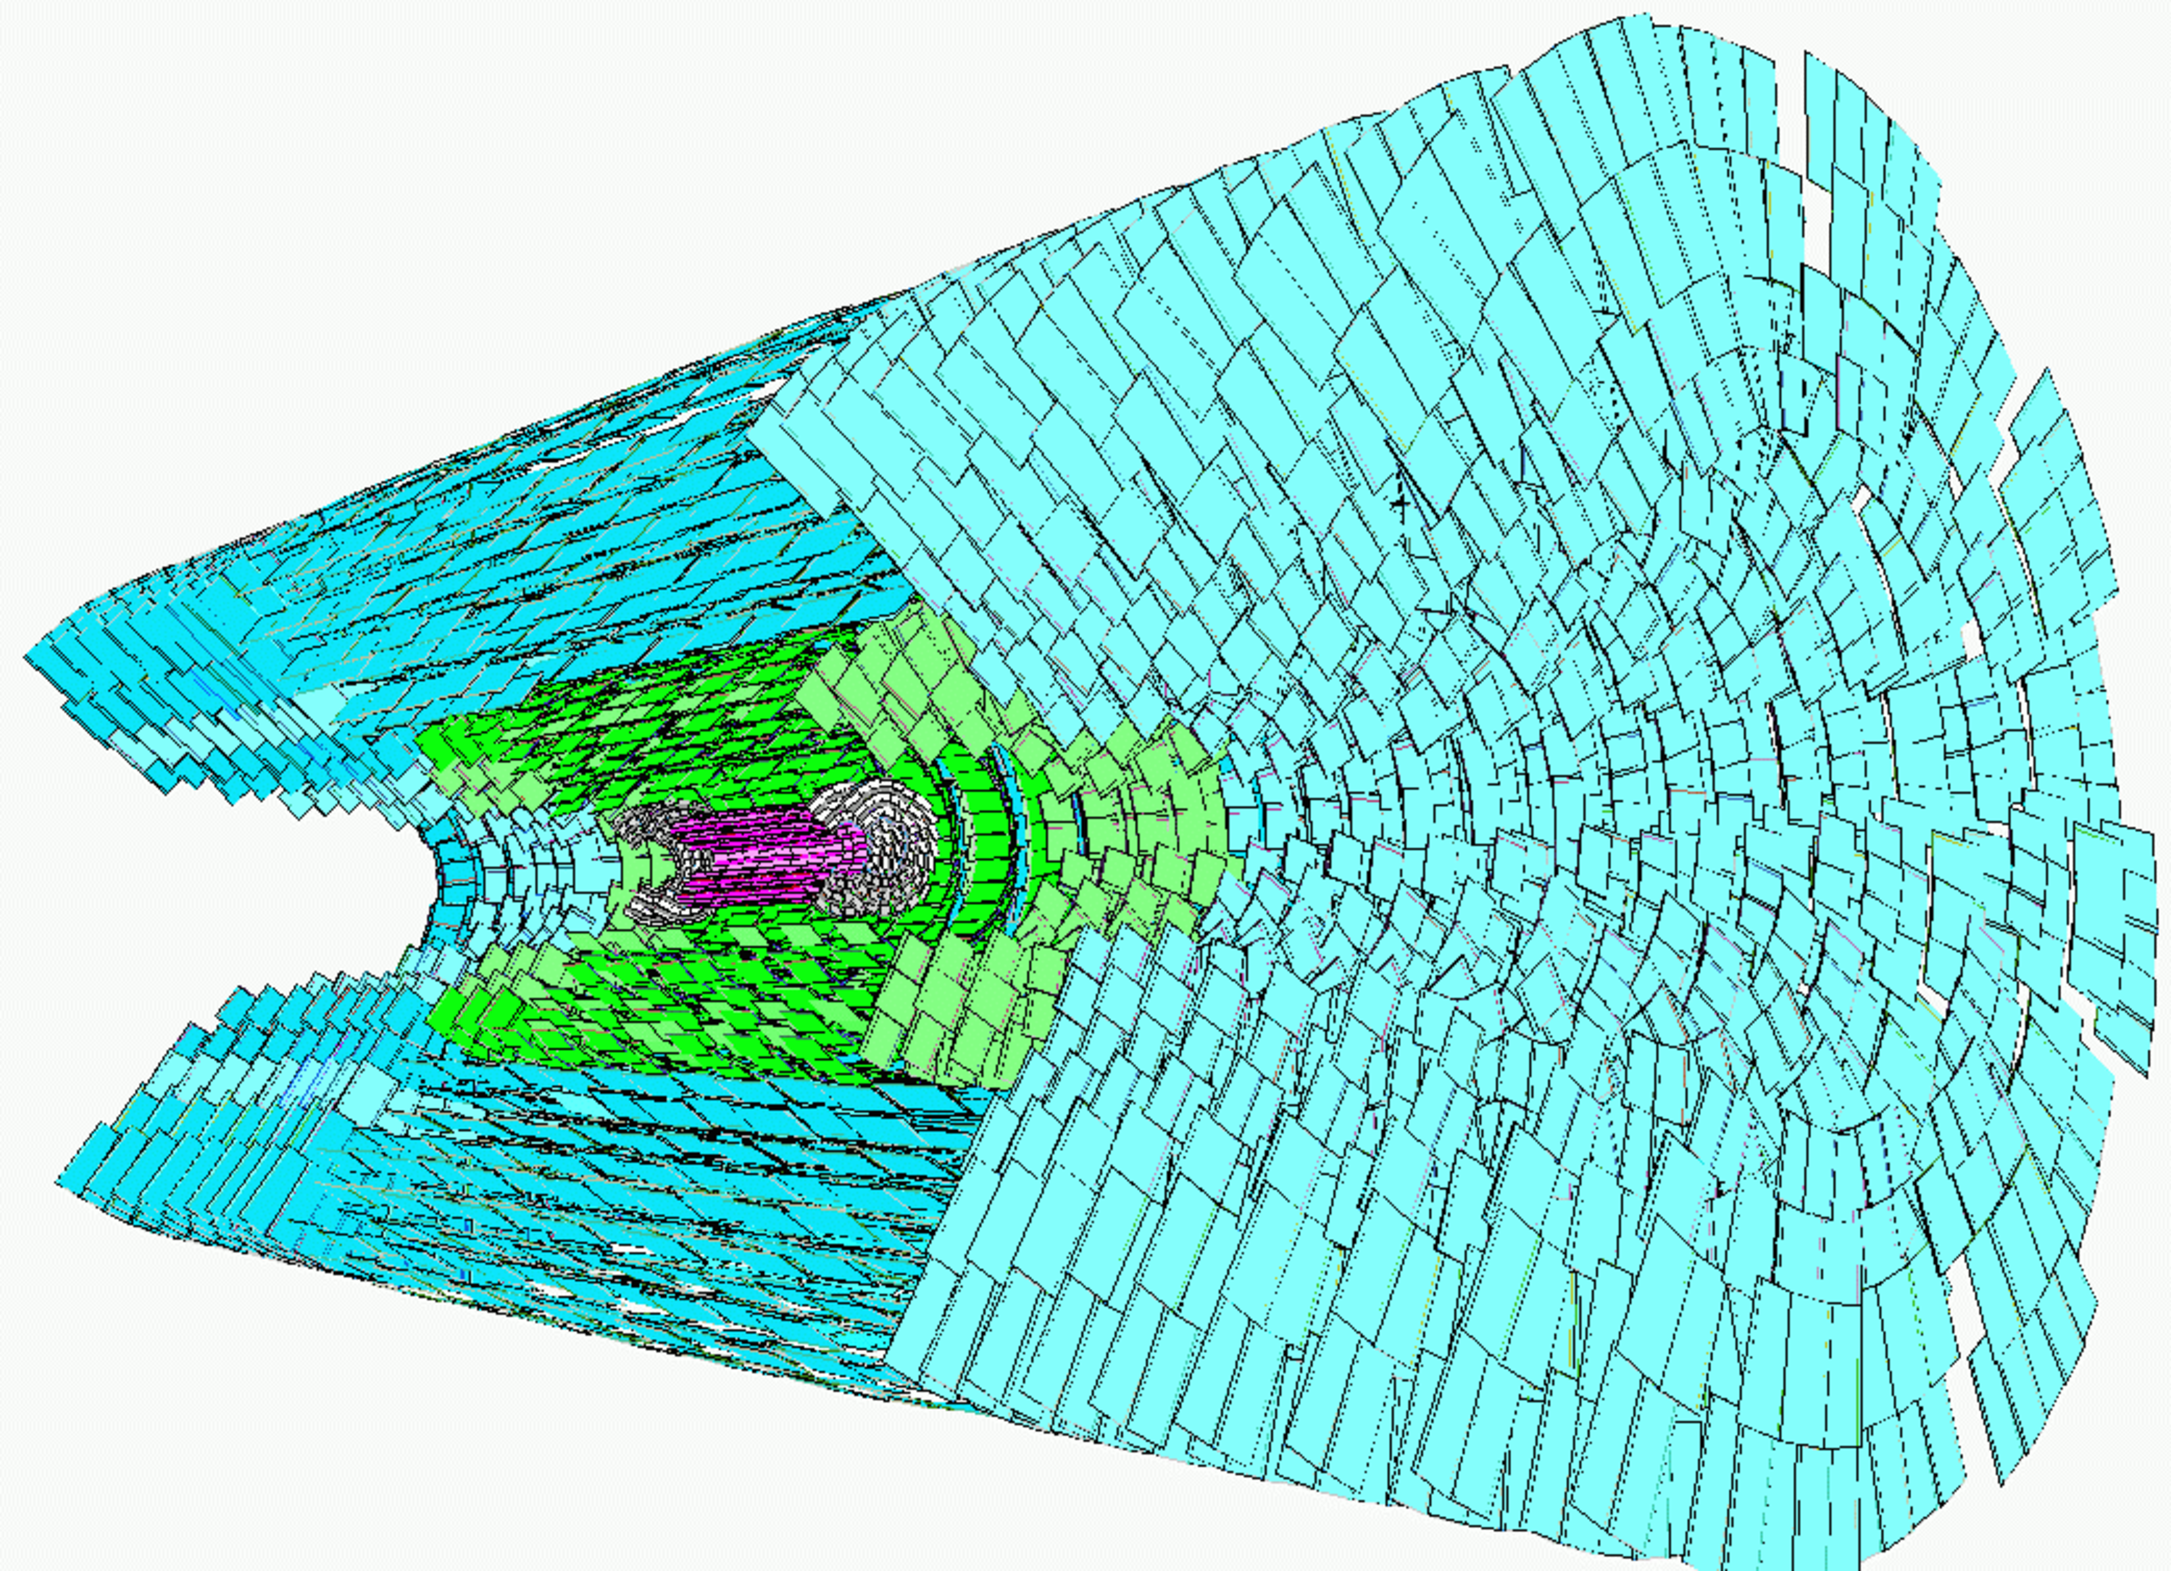
\includegraphics[width=0.75\textwidth]{detector/pics/tracker2-2.pdf}
	\end{tabular}
	\caption{Visualization of the Si-Modules of the CMS Tracker \cite{Schael:2003ca}.}
	\label{fig:Tracker_layout}
\end{figure}

\subsection{The Electromagnetic calorimeter}

The Electromagnetic Calorimeter (ECAL) is an almost hermetic, homogeneous calorimeter comprising lead tungstate ($\text{PbWO}_{4}$) crystals mounted in the central barrel part, closed by crystals in each of the two endcaps. The final design aim was to build a calorimeter as compact as possible. In order to have high hermeticity the space in between crystals has been reduced as much as possible especially in the transition region between barrel and endcaps. 
The crystal material choice was driven by the short radiation length and small Moli\`{e}re radius $R_{M}$, granting compactness and good granularity as listed on \autoref{table:CMS_PbWO4}. Other important properties of  $\text{PbWO}_{4}$ are radiation resistance and the short decaying time which allows to collect the $85\%$ of light produced by the elecromagnetic showers during the $25$ ns interval between a bunch crossing and the next one.

\begin{table}[tbh!]
	\begin{center}
		
		\begin{tabular}{ | l | c |}
			\hline
			Density  & $ 8.28$ $\text{g} /\cm^{3}$ \\ \hline
			$X_{0}$   & $0.89$ \cm \\ \hline
			Moli\`{e}re Radius $R_{M}$ 2.2 & $2.2$ \cm  \\ \hline
		\end{tabular}
		\caption{Parameters of the $\text{PbWO}_{4}$ crystals.}
		\label{table:CMS_PbWO4}
	\end{center}
\end{table}

The barrel covers a pseudo-rapidity region of $|\eta| < 1.479$ with its cylinder radius of 129 cm. It contains 61200 crystals; 360 placed in $\phi$ and $2\times85$ in $\eta$. The crystals are quasi-projective (the axes are tilted at $3^{\circ}$ with respect to the line from the nominal vertex position) and cover $0.0174$ (i.e. $\approx1^{\circ}$) in $\Delta\phi$ and $\Delta\eta$. The crystals have a front face cross-section of $\approx 22\times 22 \text{mm}^{2}$ and a length of 230 mm, corresponding to $25.8 X_{0}$. The Endcaps cover the pseudo-rapidity of $1.48 < |\eta| < 2.6$ where the $2.6\times2.6\times22 \text{cm}^{3}$ are gathered in $5\times5$ matrices called supercrystals.

In the pseudo-rapidity interval of $1.653 < |\eta| < 2.56$, as shown on \autoref{fig:ECAL_section}, a halo-ring shaped detector, called Preshower, is installed. It is a sampling calorimeter made by two distinct layers; the showering layer made of lead and the detector layer made of silicon strips capable of measuring the energy deposit of the initial part of particle showers as well as their lateral profile. The role of this detector is important whenever multiple particle showers overlap in the ECAL Endcap allowing a clear distinction of each of those showers.

The overall ECAL resolution can be parametrized as a function of the energy measured:

\begin{equation}
\dfrac{\sigma}{E}^{2} = \dfrac{S}{\sqrt{E}}^{2} + \dfrac{N}{E}^{2} + C^{2}
\end{equation}

where $S$ is the stochastic term, $N$ the noise and $C$ the constant term. The values of these
parameters are listed on \autoref{fig:ECAL_resolution}.  

\begin{figure}[tbh!]
	\centering
	\begin{tabular}{cc}
		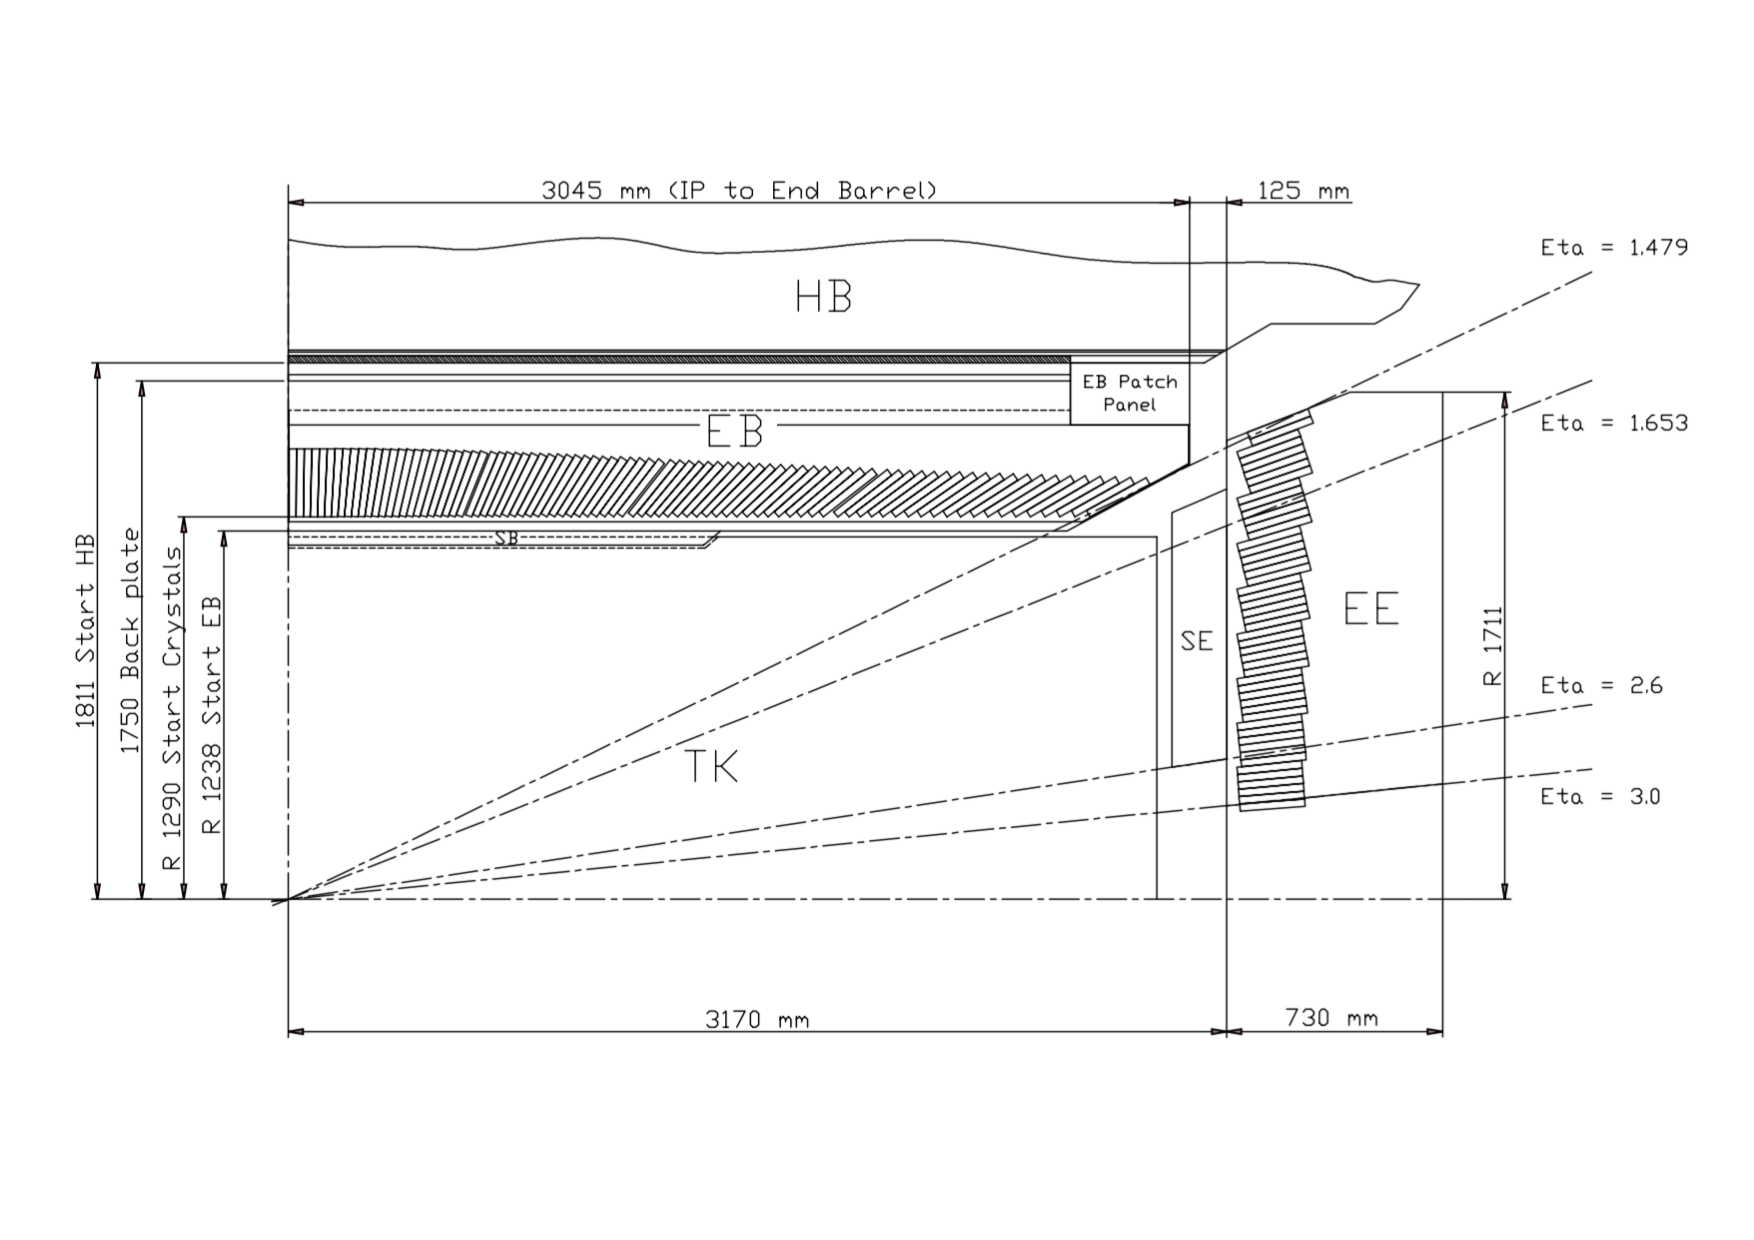
\includegraphics[width=0.75\textwidth]{detector/pics/ECAL_section.pdf}
	\end{tabular}
	\caption{Longitudinal section of the electromagnetic calorimeter (one quadrant).}
	\label{fig:ECAL_section}
\end{figure}

\begin{figure}[tbh!]
	\centering
	\begin{tabular}{cc}
		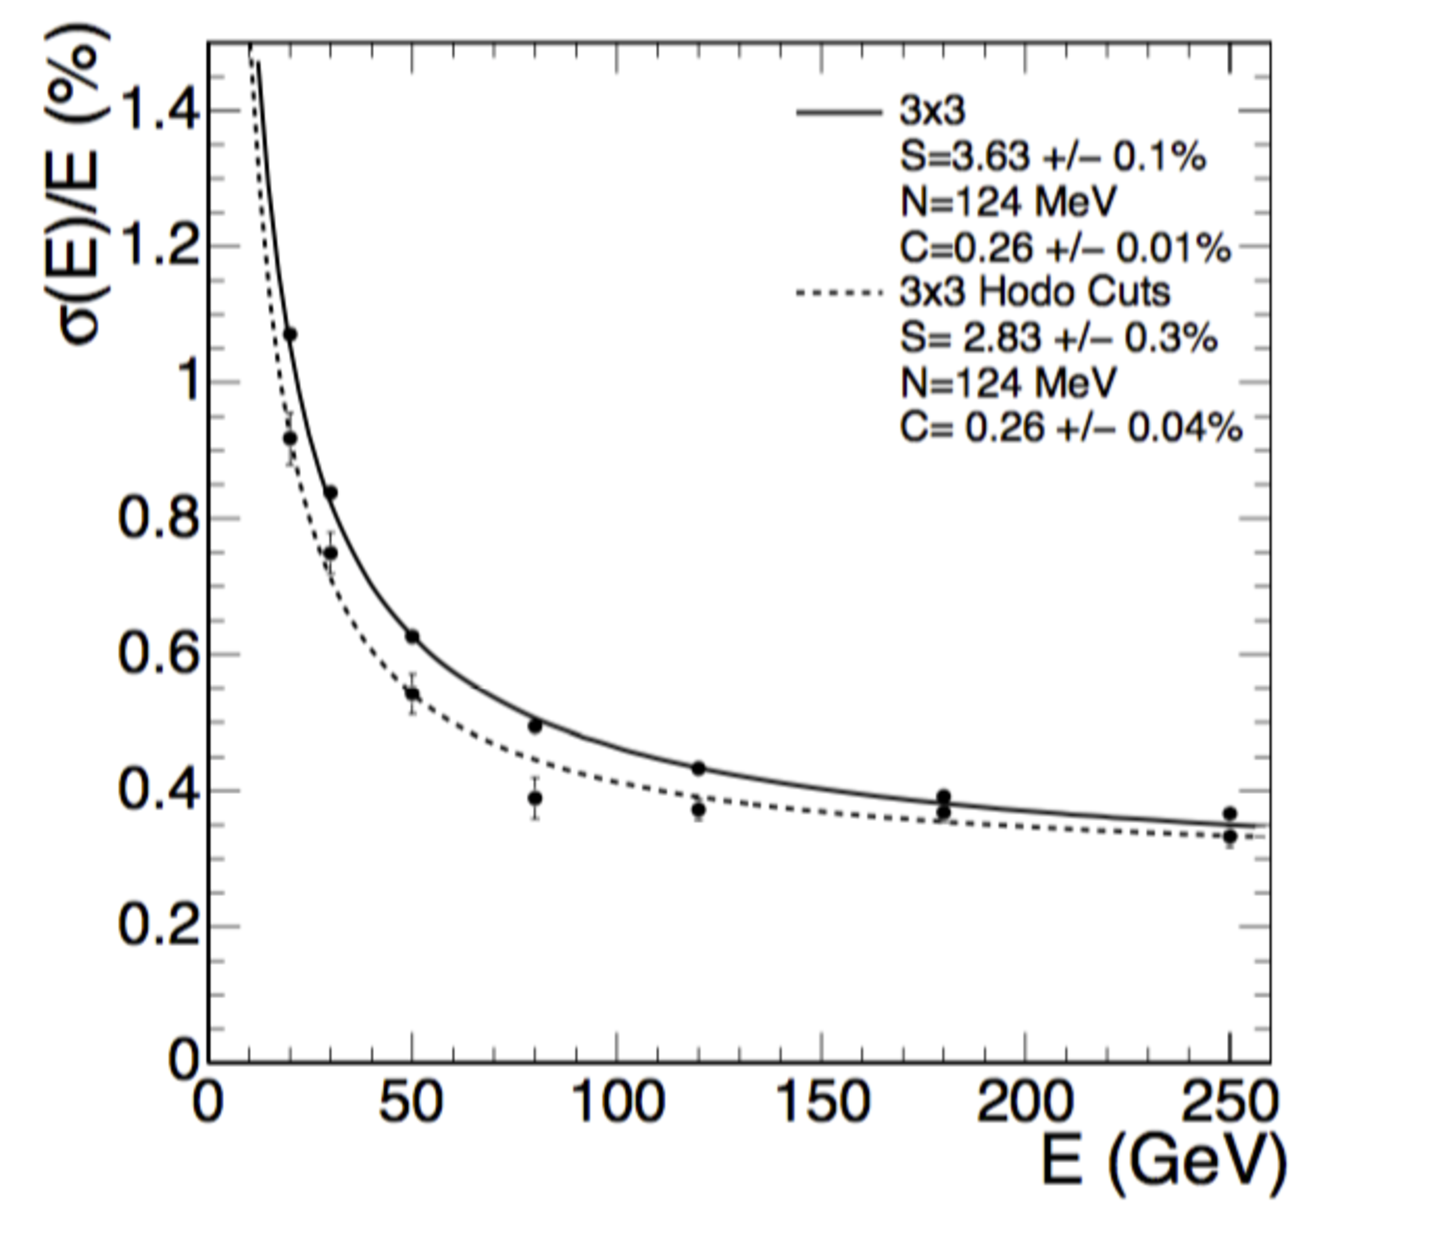
\includegraphics[width=0.75\textwidth]{detector/pics/ECAL_resolution.pdf}
	\end{tabular}
	\caption{ECAL supermodule energy resolution, $\sigma_{E}/E$, as a function of electron energy as measured from a beam test. The upper series of points correspond to events taken with a $20\times20\mm^{2}$ trigger. The lower series of points correspond to events selected to fall within a $4\times4\mm^{2}$ region. The energy was measured in an array of $3\time3$ crystals with electrons impacting the central crystal.}
	\label{fig:ECAL_resolution}
\end{figure}

\clearpage

\subsection{The Hadron calorimeter}

The Hadronic Calorimeter (HCAL) is used along side with the electromagnetic one in order to measure the energy deposit and position in the detector for hadronic jets and the missing transverse energy $\met$. The requirements for this detector are to minimize as much as possible the Gaussian tail of the resolution distribution and good containment of the hadronic showers in order to have good $\met$ reconstruction. Its design is influenced by the choice of the magnet parameters since is located inside the superconducting magnet along with the ECAL and the inner tracking system. 

The barrel region of the HCAL (HB) consists of 32 towers covering the pseudo-rapidity region $-1.4 < \eta < 1.4$, resulting in 2304 towers with a segmentation $\Delta\eta\times\Delta\phi = 0.087\times0.087$, corresponding to a $5\times5$ ECAL crystal tower. The HB is constructed in two half barrels and has a single longitudinal sampling. There are 15 brass plates, each with a thickness of about 5 cm, plus two external stainless steel plates for mechanical strength. Particles leaving the ECAL volume first see a scintillator plate with a thickness of 9 mm rather than 3.7 mm for the other plates. The light collected by the first layer is optimized to be a factor about 1.5 higher than the other scintillator plates. The radiation length $\lambda_{0}$ for the HB is $8.9\cm$.

The endcap regions of the HCAL (HE) consists of 14 $\eta$ towers with $5^{\circ}$ $\phi$ segmentation, covering the pseudo-rapidity region $1.3 < |\eta| < 3.0$. For the five innermost towers (at smaller $\eta$) the $\phi$ segmentation is $5^{\circ}$ and the $\eta$ segmentation is 0.087. For the eight outermost towers the $\phi$ segmentation is $10^{\circ}$, whilst the $\eta$ segmentation varies from 0.09 to 0.35 at highest $\eta$. The total number of HE towers is 2304. The radiation length $\lambda_{0}$ for HE is $10.0\cm$.

In order to improve the shower containment there's another calorimeter, called "Tail catcher" (HO) placed right outside the magnet. As further hermeticity improvement a "forward" calorimeter (HF) has been installed at around $11$ meters from the interaction point, covering the $\eta$ region of $3.0 < |\eta| <5.0$. This calorimeter is made of steel/quartz fibres running parallel to the beam line.

\autoref{fig:HCAL_section} shows the longitudinal section of the HCAL and the locations of its parts HB, HE, HF and HO.

The HCAL energy resolution is:

\begin{equation}
\dfrac{\sigma(E)}{E} \sim \dfrac{100\%}{\sqrt{E}}\oplus 4.5\%
\end{equation}

\begin{figure}[tbh!]
	\centering
	\begin{tabular}{cc}
		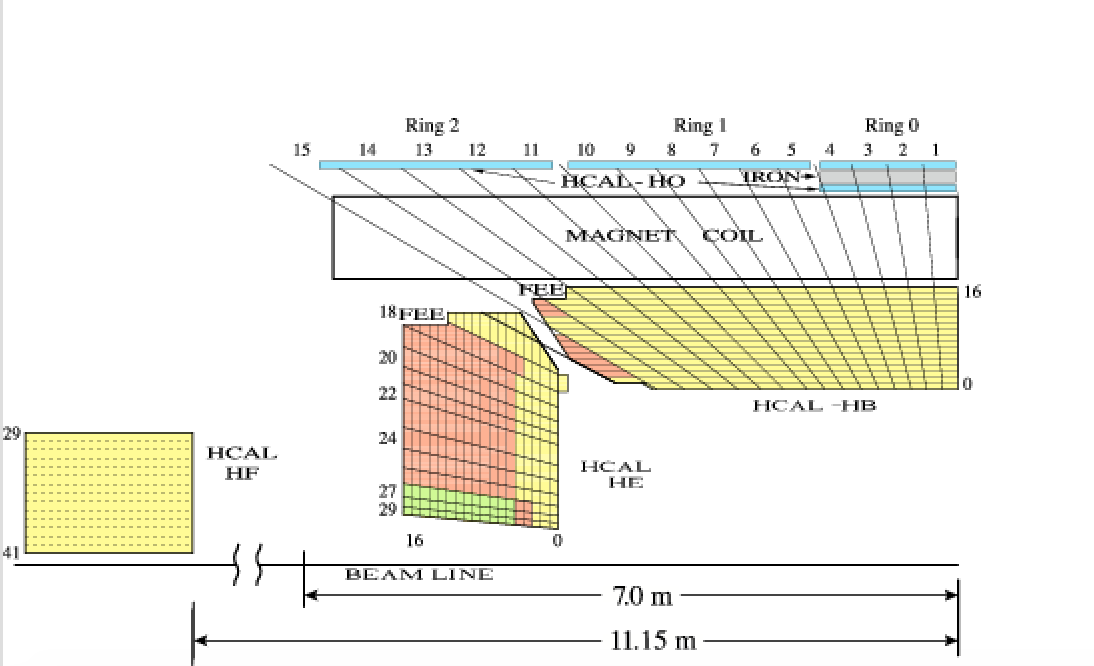
\includegraphics[width=0.75\textwidth]{detector/pics/HCAL_section.png}
	\end{tabular}
	\caption{The CMS HCAL detector (quarter slice). "FEE" indicates the locations of the Front End Electronics for HB and HE. The signals of the tower segments with the same color are added optically, to provide the HCAL "longitudinal" segmentation. HB, HE and HF are built of 36 identical azimuthal wedges\,($\Delta\phi = 20$ degrees).}
	\label{fig:HCAL_section}
\end{figure}

\autoref{fig:HCAL_resolution} shows the distribution of the jet energy resolution for different jet flavors as function of the simulate jet traverse energy \cite{Khachatryan:2016kdb}.

\begin{figure}[tbh!]
	\centering
	\begin{tabular}{cc}
		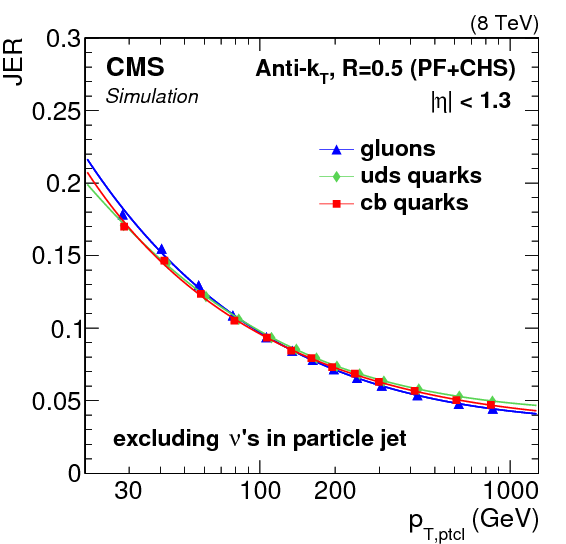
\includegraphics[width=0.50\textwidth]{detector/pics/JER_8tev_nonu.png}
		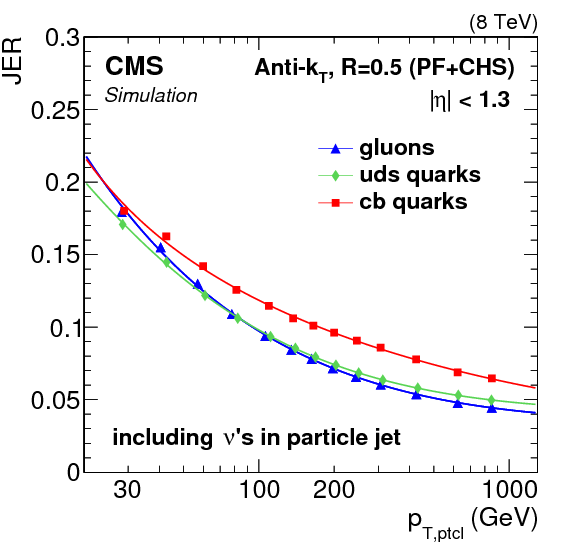
\includegraphics[width=0.50\textwidth]{detector/pics/JER_8tev_nu.png}
	\end{tabular}
	\caption{True jet energy resolution in simulation for different jet flavors in the $\gamma + \text{jet}$ sample, for jets with $| \eta | < 0.5$. The distributions are shown for particle-level jets with no neutrinos (left), and with neutrinos exceptionally included (right) to demonstrate the large fluctuations this induces for c and b jets \cite{Khachatryan:2016kdb}.}
	\label{fig:HCAL_resolution}
\end{figure}

\clearpage

\subsection{The Muon System}

\begin{figure}[tbh!]
	\centering
	\begin{tabular}{cc}
		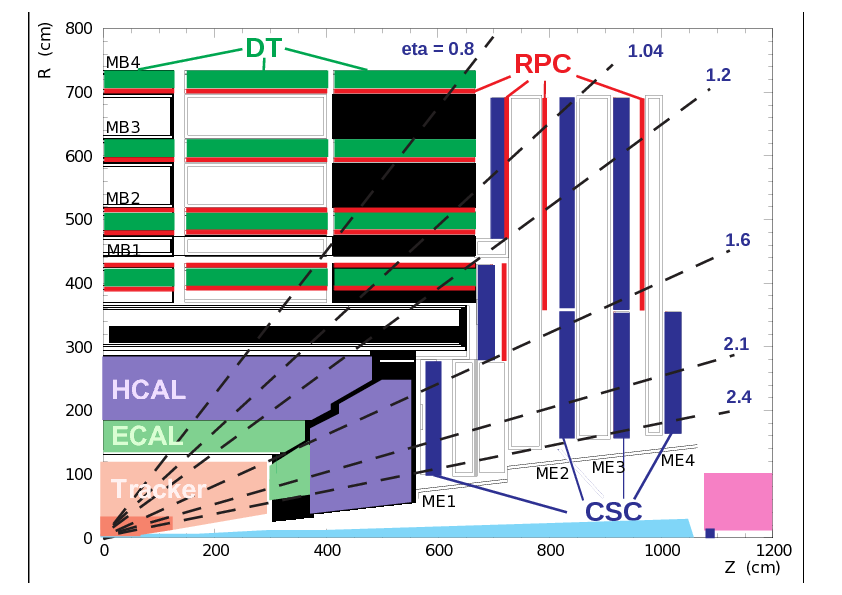
\includegraphics[width=0.75\textwidth]{detector/pics/CMS_muonsys.png}
	\end{tabular}
	\caption{Layout of one quarter of the CMS muon system for initial low luminosity running.
		The RPC system is limited to $|\eta| < 1.6$ in the endcap, and for the CSC system only the inner
		ring of the ME4 chambers have been deployed.}
	\label{fig:CMS_muonsys}
\end{figure}

Three types of gaseous detectors are used to identify and measure muons \cite{CMS:1997dma}. The choice of the detector technologies has been driven by the following reasons: the high radiation environment and the large surface area that has to be covered. Since in the barrel region ($|\eta| < 1.2$), both the muon rate and the residual magnetic field in the chambers is low, drift tube (DT) chambers are used. In the two endcaps instead, where the muon rate as well as the neutron induced background rate is high, and the magnetic field is also high, cathode strip chambers (CSC) are placed covering the pseudo-rapidity region up to $|\eta| < 2.4$. Additionally, resistive plate chambers (RPC) are used in both the barrel and the endcap regions covering a pseudo-rapidity region of $|\eta| < 2.1$. These RPCs operate in avalanche mode to ensure good performances at high rates and have double gap of 2\mm filled with gas. RPCs provide a fast response with good time resolution but with a coarser position resolution than the DTs or CSCs. RPCs can therefore identify unambiguously the correct bunch crossing \cite{Chatrchyan:2009hg}.

The DTs or CSCs and the RPCs operate within the first level trigger system, providing independent and complementary sources of information.
The layout of one quarter of the CMS muon system for the initial luminosity running is shown in \autoref{fig:CMS_muonsys}. In total, the muon system contains of order 25000 $\m^{2}$ of active detection planes, and nearly 1 million electronic channels.

\clearpage

\subsection{The Trigger System}

With a bunch crossing rate of 40 Mhz at design luminosity and the possibility to record the information for $\sim$100 Hz crossings per second, the CMS experiment needs a trigger system capable of a high rejection factor.

The CMS trigger and data acquisition system (DAQ) consist of four parts: the detector electronics, the hardware-based level 1 trigger, the readout network and the online event filter system that uses a software-based high level trigger (HLT) \cite{bib:cmstdr:trigger}.

There's a minimum transit time required for the signal to reach the level 1 trigger hardware based on the service tunnels next to the CMS experiment site, wait for the trigger response to keep or discard the event and send it back to the detectors readout apparatus. The average time needed for a single cycle is 3.2 $\mu$s. During the following time the event information is stored in a buffer waiting for the Level-1 trigger response. The trigger decisional time is less than 1 $\mu$s with a rejection power of around 1 crossing kept for every 1000. An overview of the CMS L1 trigger system is shown on \autoref{fig:CMS_trigger}.

The Level-1 decision is based on "trigger primitive" objects such as photons, electrons and muons and jets above thresholds as well as the transverse energy $E_{T}$ and the missing transverse energy \met involving the calorimetry and the muon system and a combination between these detectors. Since the Level-1 trigger is meant to take fast decisions at a high rate (the design value is 100kHz) the trigger objects are reconstructed with reduced resolution and granularity. A safe time margin of a factor of 3 is taken into account in order to cover for possible reconstruction uncertainties as well as beam and detector conditions leading to a rate of $\sim$16kHz. The design value of 100 kHz is set by the average time to transfer full detector information through the readout system.

\begin{figure}[tbh!]
	\centering
	\begin{tabular}{cc}
		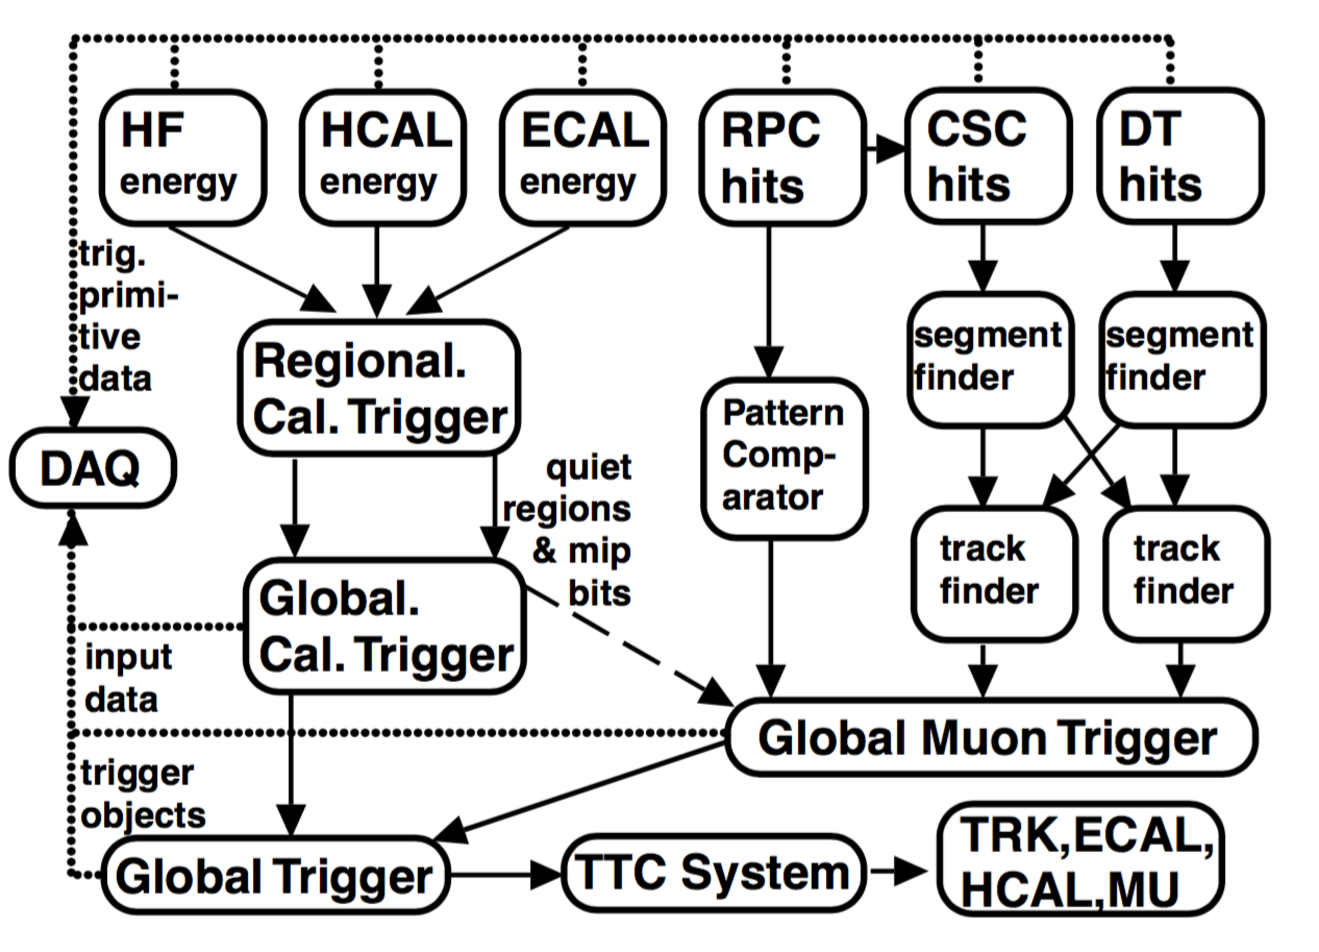
\includegraphics[width=0.75\textwidth]{detector/pics/trigger_lvl1.pdf}
	\end{tabular}
	\caption{Overview of the CMS L1 trigger system \cite{Khachatryan:2016bia}. Data from the forward (HF) and barrel (HCAL) hadronic calorimeters, and from the electromagnetic calorimeter (ECAL), are processed first regionally (RCT) and then globally (GCT). Energy deposits (hits) from the resistive-plate chambers (RPC), cathode strip chambers (CSC), and drift tubes (DT) are processed either via a pattern comparator or via a system of segment- and track-finders and sent onwards to a global muon trigger (GMT). The information from the GCT and GMT is combined in a global trigger (GT), which makes the final trigger decision. This decision is sent to the tracker (TRK), ECAL, HCAL or muon systems (MU) via the trigger, timing and control (TTC) system. The data acquisition system (DAQ) reads data from various subsystems for offline storage. MIP stands for minimum-ionizing particle.}
	\label{fig:CMS_trigger}
\end{figure}

Once an event passes the Level-1 trigger selection the data from the pipelines to the front end readout buffers waiting for a further event reconstruction. After a successful reconstruction the compressed event is sent to one processors of the available farm that runs the High Level Trigger (HLT) software. The main aim of the HLT is to gather all the informations collected in the event in order to trigger over more complex objects such as $\tau$ particles, multiple jets and multiple particle object or event reconstructed quantities in order to further reduce the event rate from $\sim$100kHz to $\sim$100Hz for mass storage.

\clearpage

\subsection{Software and Computing}

The CMS software and computing systems covers a broad range of tasks:

\begin{itemize}
	\item online and offline calibration and status reports for each of the subdetectors;
	\item management, maintenance and access of the data storage;
	\item reconstruction and analysis of data;
	\item support of the distributed computing infrastructure and software framework.
\end{itemize}

The scale of the CMS collaboration in terms of storage capabilities and networking power is orders of magnitude higher that the CERN's infrastructure capabilities \cite{CMS:2005aa}. Therefore the CMS computing model is highly distributed, with a primary "Tier-0" centered at CERN with the additional support by "Tier-1" and "Tier-2" computing centers scattered worldwide in several universities and research centers. 

\begin{figure}[tbh!]
	\centering
	\begin{tabular}{cc}
		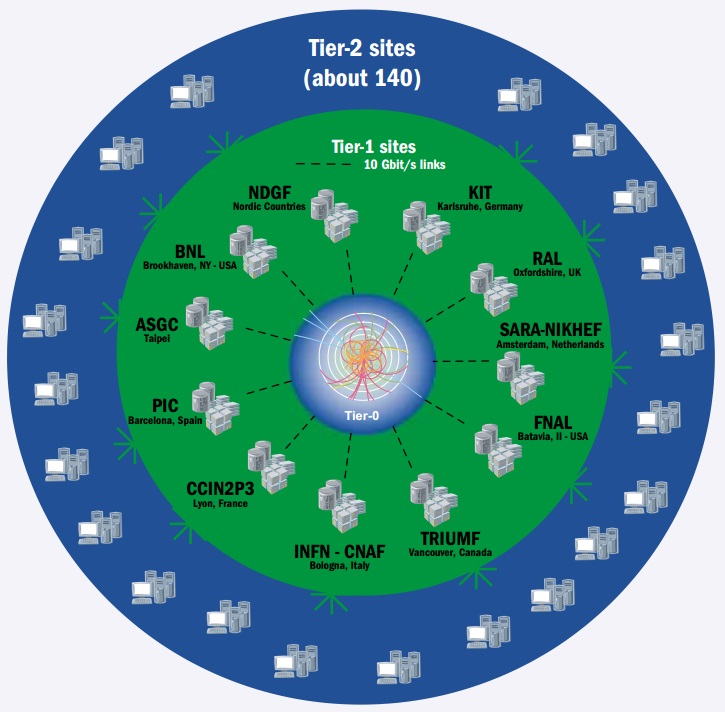
\includegraphics[width=0.75\textwidth]{detector/pics/CMS_grid.jpg}
	\end{tabular}
	\caption{Overview of the structure of the CMS Computing Grid.}
	\label{fig:CMS_grid}
\end{figure}

The scale of the CMS collaboration in terms of storage capabilities, networking power is orders of magnitude higher that the CERN's infrastructure capabilities. Therefore the CMS computing model is highly distributed consisting of four layers, or "tiers"; 0, 1, 2 and 3. Each tier provides a specific set of services.

All those facilities as shown on \autoref{fig:CMS_grid} have hierarchical structure under the Tier-0 and go under the name of "CMS Computing Grid" \cite{Charlot:2003vy}.

\subsubsection{Tier-0}

This is the CERN Data Centre, which is located in Geneva, Switzerland and also at the Wigner Research Centre for Physics in Budapest, Hungary over 1200km away. The two sites are connected by two dedicated 100 Gbit/s data links. All data from the LHC passes through the central CERN hub, but CERN provides less than $20\%$ of the total computing capacity.

Tier 0 is responsible for the safe-keeping of the raw data (first copy), first pass reconstruction, distribution of raw data and reconstruction output to the Tier 1s, and reprocessing of data during LHC down-times.

\subsubsection{Tier 1}

These are thirteen large computer centres with sufficient storage capacity and with round-the-clock support for the Grid. They are responsible for the safe-keeping of a proportional share of raw and reconstructed data, large-scale reprocessing and safe-keeping of corresponding output, distribution of data to Tier 2s and safe-keeping of a share of simulated data produced at these Tier 2s.

\subsubsection{Tier 2}

The Tier 2s are typically universities and other scientific institutes, which can store sufficient data and provide adequate computing power for specific analysis tasks. They handle analysis requirements and proportional share of simulated event production and reconstruction.

There are currently around 160 Tier 2 sites covering most of the globe.

\subsubsection{Tier 3}

Individual scientists will access these facilities through local (also sometimes referred to as Tier 3) computing resources, which can consist of local clusters in a University Department or even just an individual PC. There is no formal engagement between WLCG and Tier 3 resources. 

